\documentclass[11pt,letter]{article}\usepackage[]{graphicx}\usepackage[]{color}
%% maxwidth is the original width if it is less than linewidth
%% otherwise use linewidth (to make sure the graphics do not exceed the margin)
\makeatletter
\def\maxwidth{ %
  \ifdim\Gin@nat@width>\linewidth
    \linewidth
  \else
    \Gin@nat@width
  \fi
}
\makeatother

\definecolor{fgcolor}{rgb}{0.345, 0.345, 0.345}
\newcommand{\hlnum}[1]{\textcolor[rgb]{0.686,0.059,0.569}{#1}}%
\newcommand{\hlstr}[1]{\textcolor[rgb]{0.192,0.494,0.8}{#1}}%
\newcommand{\hlcom}[1]{\textcolor[rgb]{0.678,0.584,0.686}{\textit{#1}}}%
\newcommand{\hlopt}[1]{\textcolor[rgb]{0,0,0}{#1}}%
\newcommand{\hlstd}[1]{\textcolor[rgb]{0.345,0.345,0.345}{#1}}%
\newcommand{\hlkwa}[1]{\textcolor[rgb]{0.161,0.373,0.58}{\textbf{#1}}}%
\newcommand{\hlkwb}[1]{\textcolor[rgb]{0.69,0.353,0.396}{#1}}%
\newcommand{\hlkwc}[1]{\textcolor[rgb]{0.333,0.667,0.333}{#1}}%
\newcommand{\hlkwd}[1]{\textcolor[rgb]{0.737,0.353,0.396}{\textbf{#1}}}%

\usepackage{framed}
\makeatletter
\newenvironment{kframe}{%
 \def\at@end@of@kframe{}%
 \ifinner\ifhmode%
  \def\at@end@of@kframe{\end{minipage}}%
  \begin{minipage}{\columnwidth}%
 \fi\fi%
 \def\FrameCommand##1{\hskip\@totalleftmargin \hskip-\fboxsep
 \colorbox{shadecolor}{##1}\hskip-\fboxsep
     % There is no \\@totalrightmargin, so:
     \hskip-\linewidth \hskip-\@totalleftmargin \hskip\columnwidth}%
 \MakeFramed {\advance\hsize-\width
   \@totalleftmargin\z@ \linewidth\hsize
   \@setminipage}}%
 {\par\unskip\endMakeFramed%
 \at@end@of@kframe}
\makeatother

\definecolor{shadecolor}{rgb}{.97, .97, .97}
\definecolor{messagecolor}{rgb}{0, 0, 0}
\definecolor{warningcolor}{rgb}{1, 0, 1}
\definecolor{errorcolor}{rgb}{1, 0, 0}
\newenvironment{knitrout}{}{} % an empty environment to be redefined in TeX

\usepackage{alltt}    
\usepackage[latin1]{inputenc}
\usepackage[parfill]{parskip} % Activate to begin paragraphs with an empty line rather than an indent
\usepackage{amsmath,amsthm,amssymb,bbm} %math stuff
\usepackage{ctable}
\usepackage{placeins} % FloatBarrier
\usepackage{fancyhdr}
\usepackage{lastpage}
\usepackage{comment}
\usepackage[numbers]{natbib}   % omit 'round' option if you prefer square brackets
\bibliographystyle{plainnat}
\usepackage{setspace} %Spacing
\usepackage{graphicx,graphics}
\usepackage{booktabs,tabularx}
\usepackage{enumerate}
\usepackage{makecell}
\usepackage{xfrac}
\usepackage{color, colortbl, xcolor}
\usepackage{booktabs,dcolumn} % for use with texreg in R
\usepackage[pagebackref=true,bookmarks]{hyperref}
\hypersetup{
    unicode=false,          
    pdftoolbar=true,        
    pdfmenubar=true,        
    pdffitwindow=false,     % window fit to page when opened
    pdfstartview={FitH},    % fits the width of the page to the window
    pdftitle={001-Motivating Example},    % title
    pdfauthor={SRB},     % author
    pdfsubject={Subject},   % subject of the document
    pdfcreator={SRB},   % creator of the document
    pdfproducer={SRB}, % producer of the document
    pdfkeywords={}, % list of keywords
    pdfnewwindow=true,      % links in new window
    colorlinks=true,       % false: boxed links; true: colored links
    linkcolor=red,          % color of internal links (change box color with linkbordercolor)
    citecolor=blue,        % color of links to bibliography
    filecolor=black,      % color of file links
    urlcolor=cyan           % color of external links
}

% my commands
\newcommand{\tm}[1]{\textrm{#1}}


% fancy header commands
\renewcommand{\headrulewidth}{0.0pt}
\renewcommand{\footrulewidth}{0.0pt}
\setlength{\textheight}{9.00in}
\setlength{\textwidth}{7.00in}
\setlength{\topmargin}{-0.5in}
\setlength{\evensidemargin}{-0.25in}
\setlength{\oddsidemargin}{-0.25in}
\renewcommand{\baselinestretch}{1.2}
\makeatletter
\makeatother
\lfoot{} \cfoot{ } \rfoot{{\small{\em Page \thepage \ of \pageref{LastPage}}}}
\IfFileExists{upquote.sty}{\usepackage{upquote}}{}
\begin{document}
\pagestyle{fancy}

\title{001-Motivating Example}
\author{Body Fat Data}
\maketitle








\begin{abstract}
Identifying overweight populations is an important first step in fighting the obesity epidemic. However, accurate measure of body fat are costly and inconvenient. Therefore we are interested in determining predictors of body fat which require only a scale and a measuring tape. We analyze a dataset which contains percentage of body fat, age, weight, height and ten body circumference measurements for 251 men. We model the data using multiple linear regression and perform various model selection techniques.
\end{abstract}


\section{EDA}



\begin{knitrout}
\definecolor{shadecolor}{rgb}{0.969, 0.969, 0.969}\color{fgcolor}

{\centering 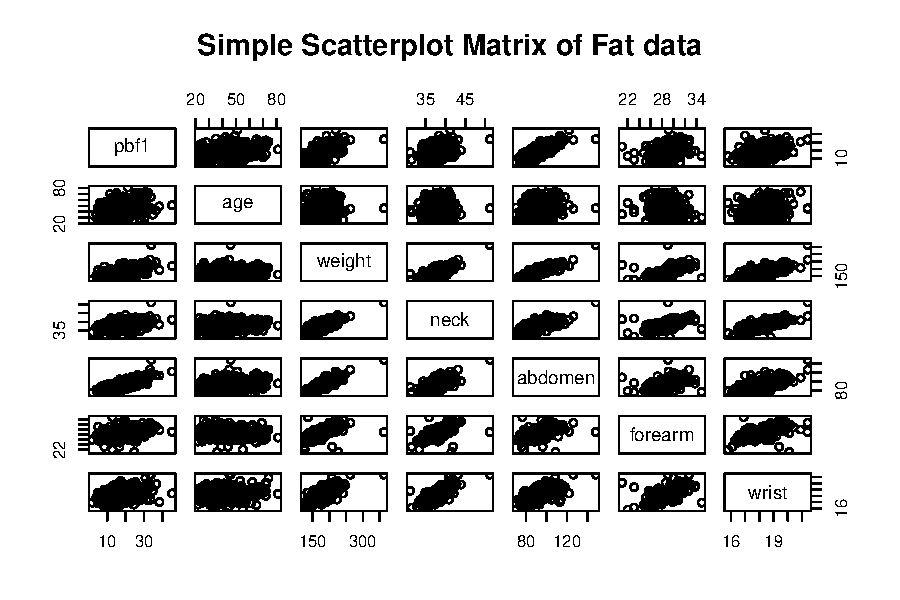
\includegraphics[width=\maxwidth]{figure/fig-pairs-1} 

}



\end{knitrout}

We will fit a model of the form
\begin{multline}
pbf1_i= \beta_0+\beta_1\tm{age}_i+\beta_2\tm{weight}_i+\beta_3\tm{height}_i+\beta_4\tm{neck}_i\\
+\beta_5\tm{chest}+\beta_6\tm{abdomen}_i+\beta_7\tm{hip}_i+\beta_8\tm{thigh}_i+\beta_9\tm{knee}_i \\
+\beta_{10}\tm{ankle}_i+ \beta_{11}\tm{bicep}_i +\beta_{12}\tm{forearm}_i +\beta_{13}\tm{wrist}_i ,  \label{eq:eq1}
\end{multline}

\FloatBarrier

\section{Results}

The parameter estimates of Model~\eqref{eq:eq1} and their standard errors are shown in Table~\ref{tab:results}

\begin{table}
\begin{center}
\begin{tabular}{l D{)}{)}{13)3}@{} }
\toprule
            & \multicolumn{1}{c}{Model 1} \\
\midrule
(Intercept) & -12.39 \; (16.18)    \\
age         & 0.06 \; (0.03)       \\
weight      & -0.07 \; (0.05)      \\
height      & -0.07 \; (0.09)      \\
neck        & -0.43 \; (0.21)^{*}  \\
chest       & -0.04 \; (0.09)      \\
abdomen     & 0.89 \; (0.08)^{***} \\
hip         & -0.20 \; (0.13)      \\
thigh       & 0.21 \; (0.13)       \\
knee        & -0.02 \; (0.22)      \\
ankle       & 0.15 \; (0.20)       \\
bicep       & 0.17 \; (0.16)       \\
forearm     & 0.42 \; (0.18)^{*}   \\
wrist       & -1.49 \; (0.49)^{**} \\
\midrule
R$^2$       & 0.74                 \\
Adj. R$^2$  & 0.73                 \\
Num. obs.   & 251                  \\
RMSE        & 3.98                 \\
\bottomrule
\multicolumn{2}{l}{\scriptsize{$^{***}p<0.001$, $^{**}p<0.01$, $^*p<0.05$}}
\end{tabular}
\caption{Multiple Linear Regression of the Body Fat Data}
\label{tab:results}
\end{center}
\end{table}


Model diagnostics are shown in Figures~\ref{fig:fig-diagnostics} and~\ref{fig:influence-plot}

\begin{knitrout}
\definecolor{shadecolor}{rgb}{0.969, 0.969, 0.969}\color{fgcolor}\begin{figure}[h]

{\centering 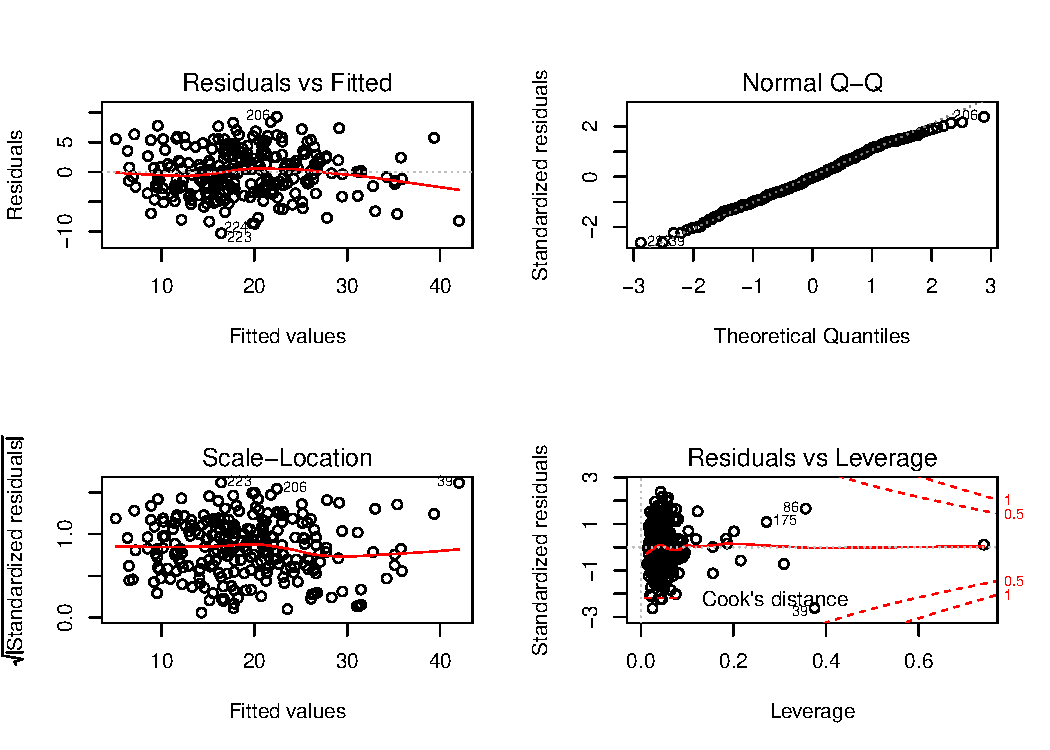
\includegraphics[width=\maxwidth]{figure/fig-diagnostics-1} 

}

\caption{Regression diagnostics for Model~\eqref{eq:eq1}}\label{fig:fig-diagnostics}
\end{figure}


\end{knitrout}

\begin{knitrout}
\definecolor{shadecolor}{rgb}{0.969, 0.969, 0.969}\color{fgcolor}\begin{figure}[h]

{\centering 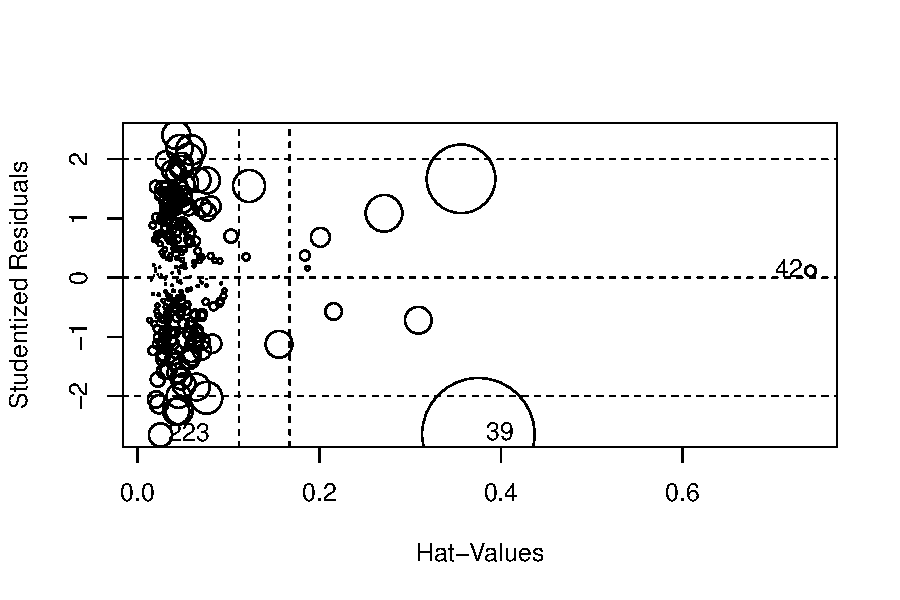
\includegraphics[width=\maxwidth]{figure/influence-plot-1} 

}

\caption{Regression influence plot for Model~\eqref{eq:eq1}}\label{fig:influence-plot}
\end{figure}


\end{knitrout}
\FloatBarrier
Look more closely at observation 42:
% latex table generated in R 3.2.0 by xtable 1.7-4 package
% Mon May 25 16:35:48 2015
\begin{table}[ht]
\centering
\begin{tabular}{rrr}
  \hline
pbf1 & weight & height \\ 
  \hline
31.70 & 205.00 & 29.50 \\ 
   \hline
\end{tabular}
\end{table}


\FloatBarrier
\section{Sensitivity Analysis}

We perform the same analysis as above, but with observation 42 removed


\begin{table}
\begin{center}
\begin{tabular}{l D{)}{)}{13)3}@{} D{)}{)}{13)3}@{} }
\toprule
            & \multicolumn{1}{c}{With obs. 42} & \multicolumn{1}{c}{Without obs. 42} \\
\midrule
(Intercept) & -12.39 \; (16.18)    & -13.85 \; (20.77)    \\
age         & 0.06 \; (0.03)       & 0.06 \; (0.03)       \\
weight      & -0.07 \; (0.05)      & -0.08 \; (0.06)      \\
height      & -0.07 \; (0.09)      & -0.06 \; (0.17)      \\
neck        & -0.43 \; (0.21)^{*}  & -0.43 \; (0.22)      \\
chest       & -0.04 \; (0.09)      & -0.04 \; (0.10)      \\
abdomen     & 0.89 \; (0.08)^{***} & 0.89 \; (0.08)^{***} \\
hip         & -0.20 \; (0.13)      & -0.20 \; (0.14)      \\
thigh       & 0.21 \; (0.13)       & 0.22 \; (0.14)       \\
knee        & -0.02 \; (0.22)      & -0.02 \; (0.23)      \\
ankle       & 0.15 \; (0.20)       & 0.15 \; (0.21)       \\
bicep       & 0.17 \; (0.16)       & 0.17 \; (0.16)       \\
forearm     & 0.42 \; (0.18)^{*}   & 0.42 \; (0.18)^{*}   \\
wrist       & -1.49 \; (0.49)^{**} & -1.49 \; (0.50)^{**} \\
\midrule
R$^2$       & 0.74                 & 0.74                 \\
Adj. R$^2$  & 0.73                 & 0.73                 \\
Num. obs.   & 251                  & 250                  \\
RMSE        & 3.98                 & 3.99                 \\
\bottomrule
\multicolumn{3}{l}{\scriptsize{$^{***}p<0.001$, $^{**}p<0.01$, $^*p<0.05$}}
\end{tabular}
\caption{Sensitivity analsysis; Multiple Linear Regression of the Body Fat Data}
\label{tab:results2}
\end{center}
\end{table}


\begin{knitrout}
\definecolor{shadecolor}{rgb}{0.969, 0.969, 0.969}\color{fgcolor}\begin{figure}[h]

{\centering 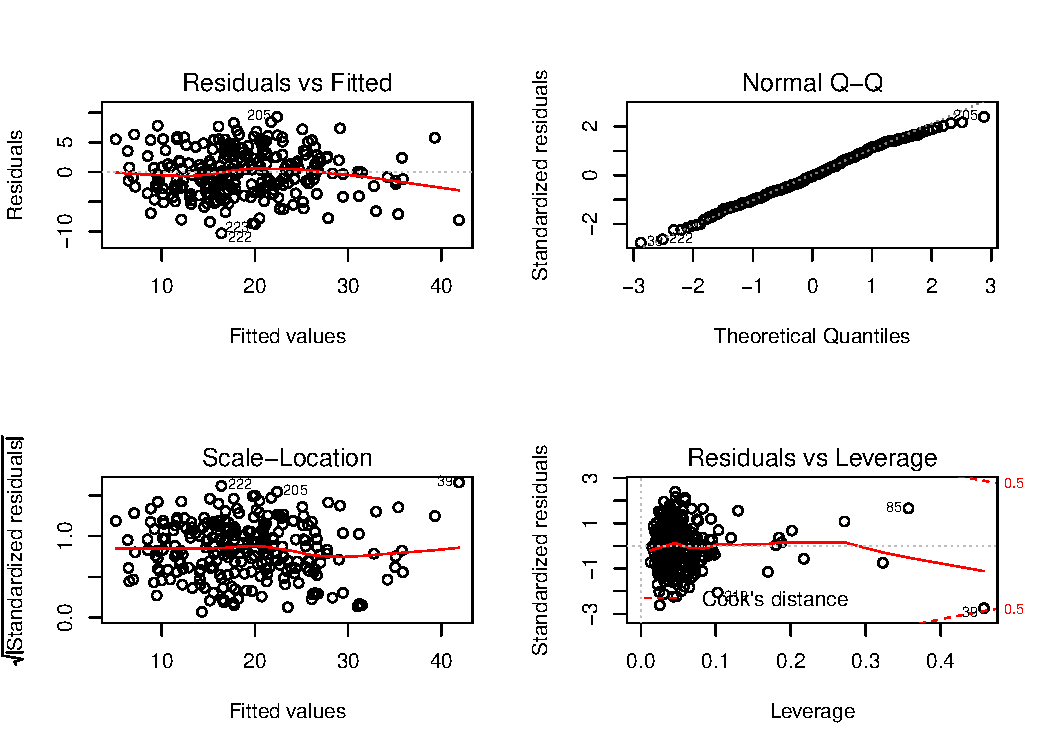
\includegraphics[width=\maxwidth]{figure/fig-diagnostics2-1} 

}

\caption{Regression diagnostics for Model~\eqref{eq:eq1}, with outliers removed}\label{fig:fig-diagnostics2}
\end{figure}


\end{knitrout}

\begin{knitrout}
\definecolor{shadecolor}{rgb}{0.969, 0.969, 0.969}\color{fgcolor}\begin{figure}[h]

{\centering 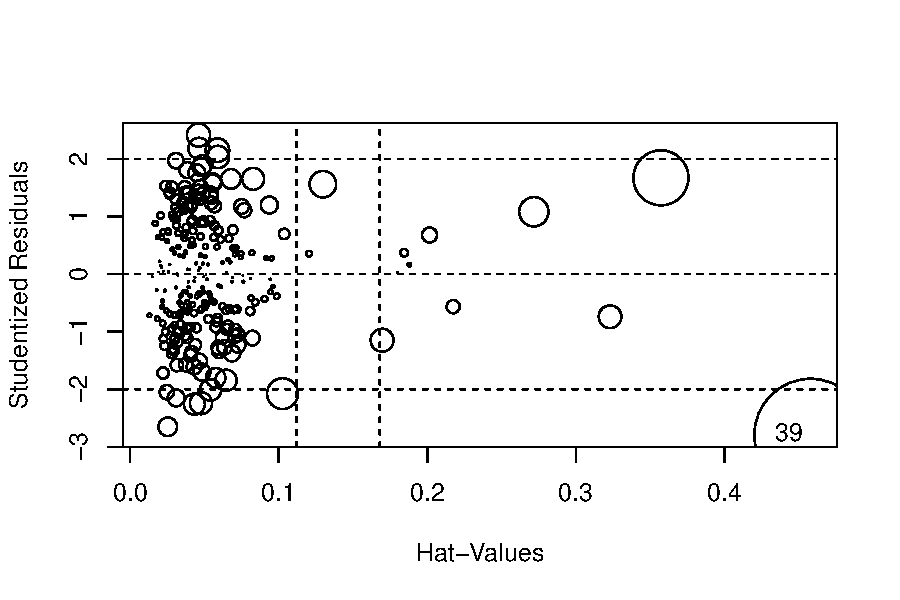
\includegraphics[width=\maxwidth]{figure/influence-plot2-1} 

}

\caption{Regression influence plot for Model~\eqref{eq:eq1}, with outliers removed}\label{fig:influence-plot2}
\end{figure}


\end{knitrout}



\end{document}
